\documentclass{article}
\usepackage[utf8]{inputenc}
\usepackage{geometry}
\usepackage{graphicx}
\usepackage{wrapfig}
\usepackage{subfig}
\usepackage{subfigure}
\usepackage{amsmath}
\usepackage{amsfonts}
\usepackage{amsthm}
\usepackage[most]{tcolorbox}
\usepackage{fancybox}
\usepackage{verbatim}
\usepackage{array}
\usepackage{latexsym}
\usepackage{alltt}
\usepackage{hyperref}
\usepackage{textcomp}
\usepackage{color}
\usepackage{float}
\usepackage{pdfpages}
\usepackage{algorithm}
\usepackage[noend]{algpseudocode}
\usepackage{multicol}
\usepackage{minted}

\usepackage[T1]{fontenc}
\usepackage{libertine}%% Only as example for the romans/sans fonts
\usepackage[scaled=0.85]{beramono}

\usepackage{colortbl}
\usepackage{pifont}
\newcommand{\cmark}{\ding{51}}
\newcommand{\xmark}{\ding{55}}

\geometry
{
 a4paper,
 left=15mm,
 top=15mm,
}

\newtcolorbox{mybox}[3][]
{
  colframe = #2!25,
  colback  = #2!10,
  coltitle = #2!20!black,  
  title    = {#3},
  #1,
}

\renewcommand\qedsymbol{$\triangle$}

\newenvironment{example}{\begin{mybox}{green}{\textbf{Example}}}{\end{mybox}}
\newenvironment{definition}[1]{\begin{mybox}{blue}{\textbf{Definition #1}}}{\end{mybox}}
\newenvironment{theorem}[1]{\begin{mybox}{red}{\textbf{Theorem #1}}}{\end{mybox}}

\def\bsq#1{%both single quotes
\lq{#1}\rq}

\makeatletter         
\renewcommand\maketitle{
{\raggedright % Note the extra {
\begin{center}
{\Large \bfseries \@title}\\[2ex] 
{\large \@author \ - \@date}\\[2ex]
\end{center}}} % Note the extra }
\makeatother

\title{CENG 242 - Chapter 2: Values and Types}
\author{Burak Metehan Tunçel}
\date{March 2022}

\begin{document}

\maketitle

\section{Types}

A \textbf{\textit{value}} is any entity that can be manipulated by a program. Values can be \textit{evaluated, stored, passed} as \textit{arguments, returned as function results}, and so on. Different programming languages support different types of values: \texttt{C} supports integers, real numbers, structures, arrays, unions, pointers to variables, and pointers to functions; \texttt{C++} supports all the above types of values plus objects. 

Most programming languages group values into \textit{types}. For instance, nearly all languages make a clear distinction between integer and real numbers. Most languages also make a clear distinction between booleans and integers: integers can be added and multiplied, while booleans can be subjected to operations like not, and, and or.

\begin{multicols}{2}
\begin{itemize}
    \item \textbf{C Types:}
        \begin{itemize}
            \item int, char, long,...
            \item float, double
            \item pointers
            \item structures: struct, union
             \item arrays
        \end{itemize}
    
    \vfill\null
    \columnbreak
    
    \item \textbf{Haskell Types:}
        \begin{itemize}
            \item Bool, Int, Float, ...
            \item Char, String
            \item tuples,(N-tuples), records
            \item lists
            \item functions
        \end{itemize}
\end{itemize}
\end{multicols}


What exactly is a type? The most obvious answer, perhaps, is that a type is a set of values. When we say that $v$ is a value of type $T$, we mean simply that $v \in T$. When we say that an expression $E$ is of type $T$, we are asserting that the result of evaluating $E$ will be a value of type $T$.

However, not every set of values is suitable to be regarded as a type. We insist that each operation associated with the type behaves uniformly when applied to all values of the type. Thus \{$false$, $true$\} is a type because the operations not, and, and or operate uniformly over the values $false$ and $true$. Also, $\{...,\ -2,\ -1,\ 0,\ +1,\ +2,...\}$ is a type because operations such as addition and multiplication operate uniformly over all these values. 

But \{13, $true$, Monday\} is not a type, since there are no useful
operations over this set of values. Thus we see that a type is characterized not only by its set of values, but also by the operations over that set of values.

Therefore we define a \textbf{\textit{type}} to be a set of values, equipped with one or more operations that can be applied uniformly to all these values. 

Every programming language supports both primitive types and composite types. Some languages also have recursive types, a recursive type being one whose values are composed from other values of the same type.

\section{Primitive Types}

A \textbf{\textit{primitive value}} is one that cannot be decomposed into simpler values. A \textbf{\textit{primitive type}} is one whose values are primitive.

Every programming language provides built-in primitive types. Some languages also allow programs to define new primitive types.

\subsection{Built-in Primitive Types}

One or more primitive types are built-in to every programming language. The choice of built-in primitive types tells us much about the programming language’s intended application area. 

Nevertheless, certain primitive types crop up in a variety of languages, often under different names. For the sake of consistency, we shall use \texttt{Boolean, Character, Integer}, and \texttt{Float} as names for the most common primitive types:
\begin{itemize}
    \item \texttt{Boolean} = \{$false$, $true$\}
    \item \texttt{Character} = \{..., \bsq a, ..., \bsq z, ..., \bsq 0, ..., \bsq 9, ..., \bsq ?, ...\}
    \item \texttt{Integer} = \{..., -2, -1, 0, +1, +2, ...\}
    \item \texttt{Float} = \{..., -1.0, ..., 0.0, ..., +1.0, ...\}
\end{itemize}

The \textbf{\textit{cardinality}} of a type $T$, written \#$T$, is the number of distinct values in $T$. For example:
\begin{itemize}
    \item \#Boolean = 2
    \item \#Character = 256 (ISO LATIN character set)
    \item \#Character = 65 536 (UNICODE character set)
\end{itemize}

\newline

If some types are implementation-defined, the behavior of programs may vary from one computer to another, even programs written in high-level languages. This gives rise to portability problems: a program that works well on one computer might fail when moved to a different computer.

One way to avoid such portability problems is for the programming language to define all its primitive types precisely. As we have seen, this approach is taken by JAVA.

\subsection{Defined Primitive Types}

Another way to avoid portability problems is to allow programs to define their own integer and floating-point types, stating explicitly the desired range and/or precision for each type. For example, the following declaration can be used in \texttt{ADA}: \lq \texttt{\textbf{type} Population \textbf{is range} 0 ... 1e10;}\rq. In ADA, we can define a completely new primitive type by enumerating its
values. Such a type is called an \textbf{\textit{enumeration type}}, and its values are called \textit{\textbf{enumerands}}.

\subsection{Discrete Primitive Types}

A \textbf{\textit{discrete primitive type}} is a primitive type whose values have a \textit{one-to-one relationship with a range of integers}.

This is an important concept in \texttt{ADA}, in which values of any discrete primitive type may be used for array indexing, counting, and so on. The discrete primitive types in \texttt{ADA} are \texttt{Boolean, Character}, integer types, and enumeration types.

Most programming languages allow only integers to be used for counting and array indexing. \texttt{C} and \texttt{C++} allow enumerands also to be used for counting and array indexing, since they classify enumeration types as integer types.


\section{Composite Types}

A \textbf{\textit{composite value}} (or \textit{data structure}) is a value that is composed from simpler values. A \textbf{\textit{composite type}} is a type whose values are composite.

Programming languages support a huge variety of composite values: tuples, structures, records, arrays, algebraic types, discriminated records, objects, unions, strings, lists, trees, sequential files, direct files, relations, etc. The variety might seem bewildering, but in fact nearly all these composite values can be understood in terms of a small number of structuring concepts, which are:
\begin{itemize}
    \item Cartesian products (tuples, records)
    \item mappings (arrays)
    \item disjoint unions (algebraic types, discriminated records, objects)
    \item recursive types (lists, trees).
\end{itemize}

Each programming language provides its own notation for describing composite types. Here, mathematical notation that is concise, standard, and suitable for defining sets of values structured as Cartesian products, mappings, and disjoint unions will be used.

\subsection{Cartesian Products, Structures, and Records}

In a \textbf{\textit{Cartesian product}}, values of several (possibly different) types are grouped into tuples.

We use the notation $(x,\ y)$ to stand for the pair whose first component is $x$ and whose second component is $y$. We use the notation $S \times T$ to stand for the set of all pairs $(x,\ y)$ such that $x$ is chosen from set $S$ and $y$ is chosen from set $T$. Formally:

\begin{equation}
    S \times T = \{(x,\ y)\ |\ x \in S;\ y \in T\}
\end{equation}

\newpage

The basic operations on pairs are:
\begin{itemize}
    \item \textbf{\textit{construction}} of a pair from two component values;
    \item \textbf{\textit{selection}} of the first or second component of a pair.
\end{itemize}

We can easily infer the cardinality of a Cartesian product:
\begin{equation}
    \text{\#}(S \times T) = \text{\#}S \times \text{\#}T
\end{equation}
This equation motivates the use of the notation ‘‘$\times$’’ for Cartesian product.

We can extend the notion of Cartesian product from pairs to tuples with any number of components. In general, the notation $S_1 \times S_2 \times ... \times S_n$ stands for the set of all $n$-tuples, such that the first component of each $n$-tuple is chosen from $S_1$, the second component from $S_2$, ..., and the $n^{th}$ component from $S_n$.

C \texttt{struct}, Pascal \texttt{record}, functional languages \texttt{tuple}
\begin{multicols}{3}

\textbf{in C:} \texttt{string} $\times$ \texttt{int}

\begin{minted}
[
%frame=lines,
%framesep=2mm,
baselinestretch=1.2,
bgcolor=lightgray,
fontsize=\footnotesize,
%linenos
]
{c}
struct Person {
    char name[20];
    int no;
} x = {" Osman Hamdi " ,23141};
\end{minted}

\vfill\null
\columnbreak

\textbf{in Haskell:} \texttt{string} $\times$ \texttt{int}   
\begin{minted}
[
%frame=lines,
%framesep=2mm,
baselinestretch=1.2,
bgcolor=lightgray,
fontsize=\footnotesize,
%linenos
]
{haskell}
type People = (String, Int)
...
x = ("Osman Hamdi", 23141)::People
\end{minted}

\vfill\null
\columnbreak

\textbf{in Python:} \texttt{string} $\times$ \texttt{int} 
\begin{minted}
[
%frame=lines,
%framesep=2mm,
baselinestretch=1.2,
bgcolor=lightgray,
fontsize=\footnotesize,
%linenos
]
{py}
x = ("Osman Hamdi", 23141)
type (x)
<type 'tuple'>
\end{minted}
\end{multicols}

A special case of a Cartesian product is one where all tuple components are chosen from the same set. The tuples in this case are said to be \textbf{\textit{homogeneous}}. For example:
\begin{equation}
    S^2 = S \times S
\end{equation}
means the set of homogeneous pairs whose components are both chosen from set $S$. More generally we write:
\begin{equation}
    S^n = S \times S \times \cdots \times S
\end{equation}
to mean the set of homogeneous $n$-tuples whose components are all chosen from set $S$.

The cardinality of a set of homogeneous $n$-tuples is given by:
\begin{equation}
    \text{\#}(S^n) = (\text{\#}S)^n
\end{equation}
This motivates the superscript notation.

Finally, let us consider the special case where $n = 0$. Equation 5 tells us that $S_0$ should have exactly one value. This value is the empty tuple $()$, which is the unique tuple with no components at all. We shall find it useful to define a type that has the empty tuple as its only value:
\begin{equation}
    \text{Unit} = \{()\}
\end{equation}
This type’s cardinality is:
\begin{equation}
    \text{\#Unit} = 1
\end{equation}
Note that Unit is \textit{not} the empty set (whose cardinality is 0). Unit corresponds to the type named \texttt{\textbf{void}} in \texttt{C}, \texttt{C++}, and \texttt{JAVA}, to the type \textbf{null record} in \texttt{ADA}, and to the  \texttt{\textbf{None}} in \texttt{Python}.

\subsection{Mappings, Arrays, and Functions}

The notion of a \textbf{\textit{mapping}} from one set to another is extremely important in programming languages. This notion in fact underlies two apparently different language features: \textit{arrays} and \textit{functions}.

We write:
\begin{equation}
    m : S \rightarrow T
\end{equation}
to state that $m$ is a mapping from set $S$ to set $T$. In other words, $m$ maps every value in $S$ to a value in $T$. (Read the symbol ‘‘$\rightarrow$’’ as ‘‘maps to’’.)

If $m$ maps value $x$ in set $S$ to value $y$ in set $T$, we write $y = m(x)$. The value $y$ is called the image of $x$ under $m$.

Two different mappings from $S = \{u,\ v\}$ to $T = \{a,\ b,\ c\}$ are illustrated in Figure 1. We use notation such as $\{u \rightarrow a,\ v \rightarrow c\}$ to denote the mapping that maps $u$ to $a$ and $v$ to $c$.

\begin{figure}[h!]
    \centering
    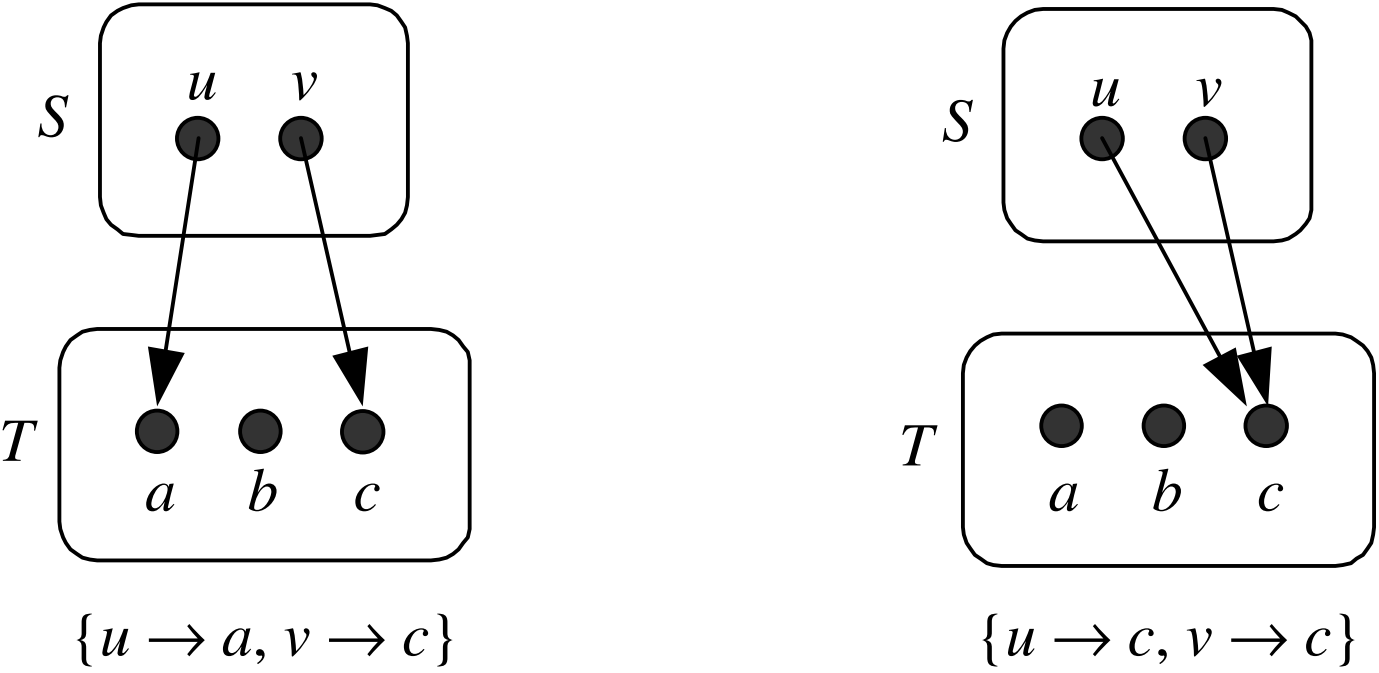
\includegraphics[width=.5\textwidth]{img/Fig2.2.png}
    \caption{Two different mappings in $S \rightarrow T$}
    \label{fig:my_label}
\end{figure}

The notation $S \rightarrow T$ stands for the set of all mappings from $S$ to $T$. Formally:
\begin{equation}
    S \rightarrow T = \{m\ |\ x \in S \Rightarrow m(x) \in T\}
\end{equation}
This is illustrated in Figure 2.

\begin{figure}[h!]
    \centering
    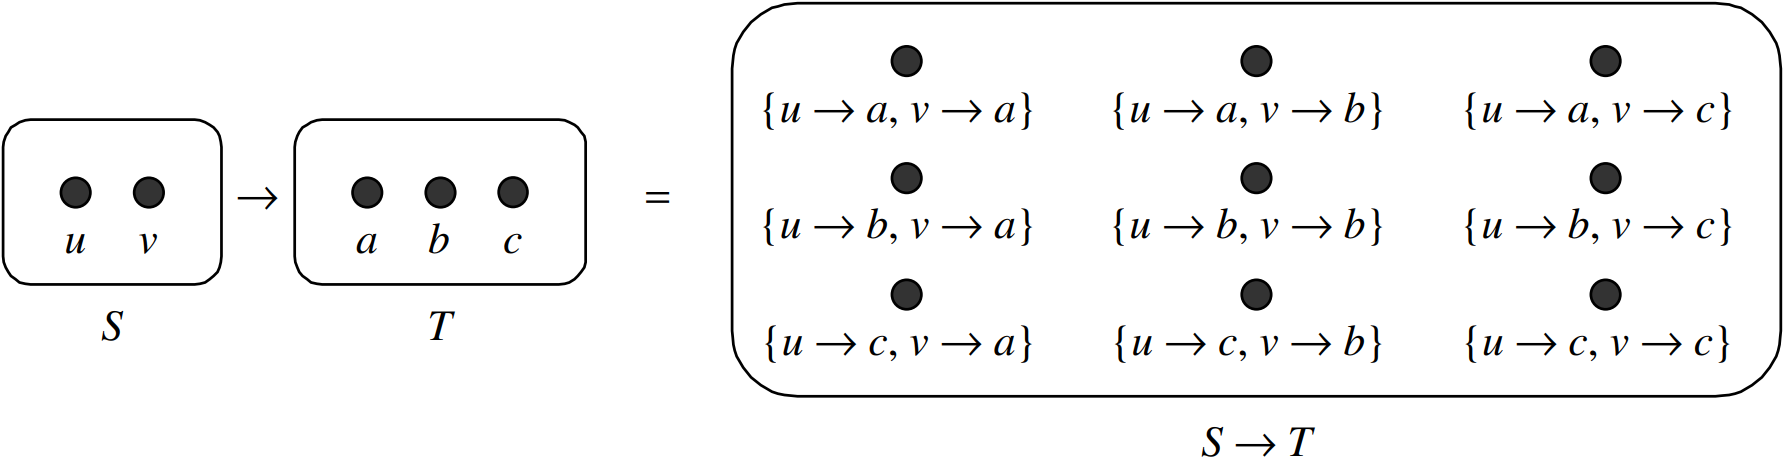
\includegraphics[width=.5\textwidth]{img/Fig2.3.png}
    \caption{Set of all mappings in $S \rightarrow T$}
    \label{fig:my_label}
\end{figure}

Let us deduce the cardinality of $S \rightarrow T$. Each value in $S$ has \#$T$ possible images under a mapping in $S \rightarrow T$. There are \#$S$ such values in $S$. Therefore there are \#$T$ $\times$ \#$T$ $\times \cdots \times$ \#$T$ possible mappings (\#$S$ copies of \#$T$ multiplied together). In short:
\begin{equation}
    \text{\#}(S \rightarrow T) = (\text{\#}T)^{\text{\#}S}
\end{equation}

An \textbf{\textit{array}} is an indexed sequence of components. An array has one component of type $T$ for each value in type $S$, so the array itself has type $S \rightarrow T$. The \textbf{\textit{length}} of the array is its number of components, which is \#$S$. Arrays are found in all imperative and object-oriented languages.

The type $S$ must be finite, so an array is a \textit{finite} mapping. In practice, $S$ is always a range of consecutive values, which is called the array’s \textit{\textbf{index range}}. The limits of the index range are called its \textbf{\textit{lower bound}} and \textbf{\textit{upper bound}}.

The basic operations on arrays are:
\begin{itemize}
    \item \textbf{\textit{construction}} of an array from its components;
    \item \textbf{\textit{indexing}}, i.e., selecting a particular component of an array, given its index.
\end{itemize}
The index used to select an array component is a computed value. Thus array indexing differs fundamentally from Cartesian-product selection (where the component to be selected is always explicit).

\texttt{C} and \texttt{C++} restrict an array’s index range to be a range of integers whose lower bound is zero. ($S$ is integers whose lower bound is 0.)

Mappings occur in programming languages, not only as arrays, but also as \textbf{\textit{function procedures}} (more usually called simply \textit{functions}). We can implement a mapping in $S \rightarrow T$ by means of a function procedure, which takes a value in $S$ (the \textbf{\textit{argument}}) and computes its image in $T$ (the \textbf{\textit{result}}). Here the set $S$ is not necessarily finite.

\subsubsection{Array and Function Difference}

\begin{multicols}{2}
\textbf{Arrays:}
\begin{itemize}
    \item Values stored in memory
    \item Restricted: only integer domain
    \item double $\rightarrow$ double ?
\end{itemize}

\vfill\null
\columnbreak

\textbf{Functions:}
\begin{itemize}
    \item Defined by algorithms
    \item Efficiency, resource usage
    \item All types of mappings possible
    \item Side effect, output, error, termination problem.
\end{itemize}
\end{multicols}

\subsection{Disjoint Unions, Discriminated Records, and Objects}

Another kind of composite value is the \textbf{\textit{disjoint union}}, whereby a value is chosen from one of several (usually different) sets.

We use the notation $S + T$ to stand for a set of disjoint-union values, each of which consists of a \textbf{\textit{tag}} together with a \textbf{\textit{variant}} chosen from either set $S$ or set $T$. The tag indicates the set from which the variant was chosen. Formally:
\begin{equation}
    S + T = \{left\ x\ |\ x \in S\} \cup \{right\ y\ |\ y \in T\}
\end{equation}
Here $left\ x$ stands for a disjoint-union value with tag $left$ and variant $x$ chosen from $S$, while $right\ x$ stands for a disjoint-union value with tag $right$ and variant $y$ chosen from $T$. This is illustrated in Figure 2.4.
\begin{figure}[h!]
    \centering
    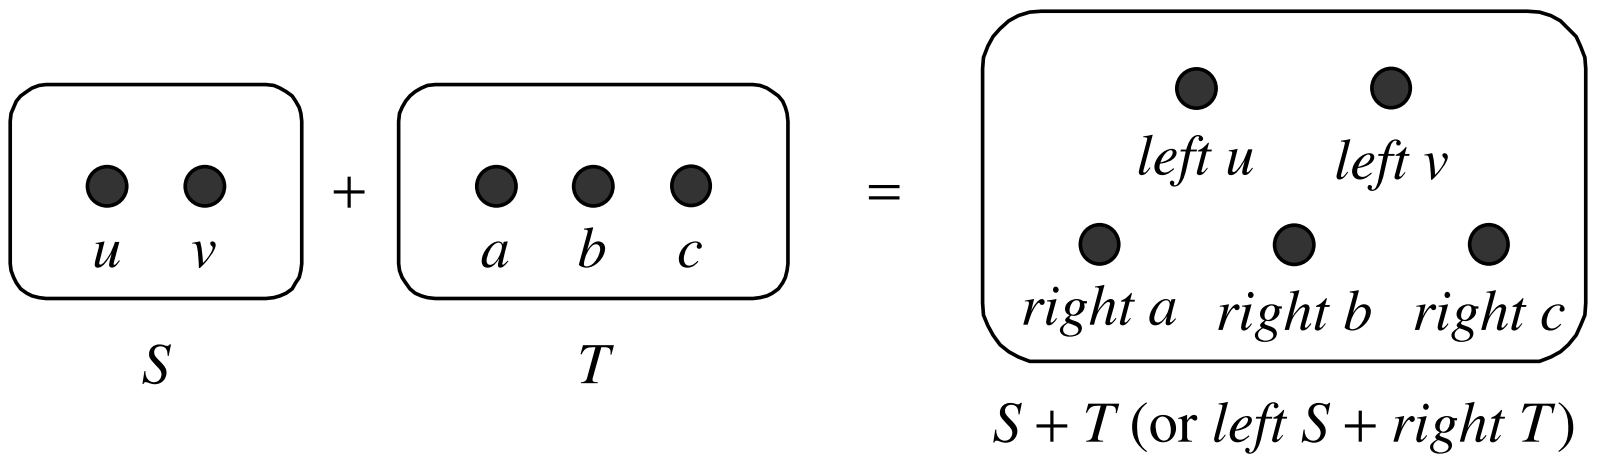
\includegraphics[width=.5\textwidth]{img/Fig2.4.png}
    \caption{Disjoint union of sets $S$ and $T$}
    \label{fig:my_label}
\end{figure}

When we wish to make the tags explicit, we will use the notation $left\ S + right\ T$:
\begin{equation}
    left\ S + right\ T = \{left\ x\ |\ x \in S\} \cup \{right\ y\ |\ y \in T\}
\end{equation}
When the tags are irrelevant, we will still use the simpler notation $S + T$.

Note that the tags serve only to distinguish the variants. They must be distinct, but otherwise they may be chosen freely. 

The basic operations on disjoint-union values in $S + T$ are:
\begin{itemize}
    \item \textbf{\textit{construction}} of a disjoint-union value, by taking a value in either $S$ or $T$ and tagging it accordingly;
    \item \textbf{\textit{tag test}}, determining whether the variant was chosen from $S$ or $T$;
    \item \textbf{\textit{projection}} to recover the variant in $S$ or the variant in $T$ (as the case may be).
\end{itemize}
For example, a tag test on the value $right\ b$ determines that the variant was chosen from $T$, so we can proceed to project it to recover the variant $b$.

We can easily infer the cardinality of a disjoint union:
\begin{equation}
    \text{\#}(S + T) = \text{\#}S + \text{\#}T
\end{equation}
This motivates the use of the notation ‘‘$+$’’ for disjoint union.

We can extend disjoint union to any number of sets. In general, the notation $S_1 + S_2 + \cdots + S_n$ stands for the set in which each value is chosen from one of $S_1,\ S_2,\ \cdots$, or $S_n$.

The functional language \texttt{HASKELL} has \textbf{\textit{algebraic types}}, which we can understand in terms of disjoint unions. In fact, the \texttt{HASKELL} notation is very close to our mathematical disjoint-union notation.\newline


How should we understand \textbf{\textit{objects}}? Simplistically we could view each object of a particular class as a tuple of components. However, any object-oriented language allows objects of different classes to be used interchangeably (to a certain extent), and therefore provides an operation to test the class of a particular object. Thus each object must have a tag that identifies its class. So we shall view each object as a \textit{tagged} tuple.


It is \textit{important not to confuse disjoint union with ordinary set union}. The tags in a disjoint union $S + T$ allow us to test whether the variant was chosen from $S$ or $T$. This is not necessarily the case in the ordinary union $S \cup T$. In fact, if $T = \{a,\ b,\ c\}$, then:
\begin{align}
    T \cup T &= \{a,\ b,\ c\} = T\\
    T + T &= \{left\ a,\ left\ b,\ left\ c,\ right\ a,\ right\ b,\ right\ c\} \neq T
\end{align}

The \textbf{unions} of C and C++ are not disjoint unions, since they have no tags. This obviously makes tag test impossible, and makes projection unsafe. In practice, therefore, C programmers enclose each union within a structure that also contains a tag.

\subsection{Power Set}

The set of all subsets. $\mathcal{P}(S) = \{T\ |\ T \subseteq S\}$. Cardinality of set \#$\mathcal{P}(S) = 2^{\text{\#}S}$ \newpage


\section{Recursive Types}

A \textbf{\textit{recursive type}} is one defined in terms of itself. In this section we discuss two common recursive types, lists and strings, as well as recursive types in general.

\subsection{Lists}

A \textbf{\textit{list}} is a sequence of values. A list may have any number of components, including none. The number of components is called the \textbf{\textit{length}} of the list. The unique list with no components is called the \textbf{\textit{empty list}}.

A list is \textbf{\textit{homogeneous}} if all its components are of the same type; otherwise it is \textbf{\textit{heterogeneous}}. 

Typical list operations are:
\begin{itemize}
    \item length
    \item emptiness test
    \item head selection (i.e., selection of the list’s first component)
    \item tail selection (i.e., selection of the list consisting of all but the first component)
    \item concatenation
\end{itemize}

Suppose that we wish to define a type of \textit{integer-lists}, whose values are lists of integers. We may define an integer-list to be a value that is either empty or a pair consisting of an integer (its head) and a further integer-list (its tail). This definition is recursive. We may write this definition as a set equation:
\begin{equation}
    \texttt{Integer-List} = nil\ \texttt{Unit} + cons(\texttt{Integer} × \texttt{Integer-List})
\end{equation}
or, in other words:
\begin{equation}
    \texttt{Integer-List} = \{nil()\} \cup \{cons(i, l)\ |\ i \in \texttt{Integer};\ l \in \texttt{Integer-List}\}
\end{equation}
where we have chosen the tags \textit{nil} for an empty list and \textit{cons} for a nonempty list. Henceforth we shall abbreviate \textit{nil}() to \textit{nil}.

\textbf{Polymorphic lists:} a single definition defines lists of many types. So, the general idea:
\begin{align}
    &L = \text{Unit} + (T \times L) &\texttt{List} \alpha = \alpha \times (\texttt{List} \alpha) + \{\textit{empty}\}
\end{align}
has a \textit{least solution} for \textit{L} that corresponds to the set of all finite lists of values chosen from \textit{T}. Every other solution is a superset of the least solution.

Lists (or sequences) are so ubiquitous that they deserve a notation of their
own: $T^*$ stands for the set of all finite lists of values chosen from $T$. Thus:
\begin{equation}
    T^* = \text{Unit} + (T \times T^*)
\end{equation}

In imperative languages (such as \texttt{C, C++}, and \texttt{ADA}), recursive types must be defined in terms of pointers. In functional languages (such as \texttt{HASKELL}) and in some object-oriented languages (such as \texttt{JAVA}), recursive types can be defined directly.

\subsection{Strings}

A \textbf{\textit{string}} is a sequence of characters. A string may have any number of characters, including none. The number of characters is called the \textbf{\textit{length}} of the string. The unique string with no characters is called the \textbf{\textit{empty string}}.

Strings are supported by all modern programming languages. Typical string operations are:
\begin{itemize}
    \item length
    \item equality comparison
    \item lexicographic comparison
    \item character selection
    \item substring selection
    \item concatenation
\end{itemize}

How should we classify strings? No consensus has emerged among programming language designers. 
\begin{itemize}
    \item One approach is to classify strings as \textit{primitive values}. 
    \item Another approach is to treat strings as \textit{arrays of characters}.
    \item A slightly different and more flexible approach is to treat strings as \textit{pointers to arrays of characters}.
    \item In a programming language that supports lists, the most natural approach is to treat strings as \textit{lists of characters}.
    \item In an object-oriented language, the most natural approach is to treat strings as \textit{objects}.
\end{itemize}

\subsection{Recursive Types in General}

As we have seen, a \textit{recursive type} is one defined in terms of itself. Values of a recursive type are composed from values of the same type.

In general, the set of values of a recursive type, \textit{R}, will be defined by a recursive set equation of the form:
\begin{equation}
    R = ... + (...R...R...)
\end{equation}
A recursive set equation may have many solutions. Fortunately, a recursive set equation always has a \textit{least solution} that is a subset of every other solution. In computation, the least solution is the one in which we are interested.

The cardinality of a recursive type is \textit{infinite}, even if every individual value of the type is finite.


\section{Type Systems}

A programming language’s \textbf{\textit{type system}} groups values into types. This allows programmers to describe data effectively. It also helps prevent programs from performing nonsensical operations, such as multiplying a string by a boolean. Performing such a nonsensical operation is called a \textbf{\textit{type error}}.

\subsection{Static vs Dynamic Typing}

Types are required to provide data processing, integrity checking, efficiency, access controls. Type compatibility on operators is essential. Before any operation is to be performed, the types of its operands must be checked in order to prevent a type error. For example, before an integer multiplication is performed, both operands must be checked to ensure that they are integers.  Such checks are called \textbf{\textit{type checks}}.

The type check must be performed before the operation itself is performed. However, there may still be some freedom in the timing: the type check could be performed either at \textit{compile-time} or at \textit{run-time}. This seemingly pragmatic issue in fact underlies an important classification of programming languages, into statically typed and dynamically typed languages.

\begin{itemize}
    \item In a \textbf{\textit{statically typed}} language, each variable and each expression has a \textit{fixed type} (which is either explicitly stated by the programmer or inferred by the compiler). Using this information, all operands can be type-checked \textit{at compile-time}.
    \item In a \textbf{\textit{dynamically typed}} language, values have fixed types, but variables and expressions have no fixed types. Every time an operand is computed, it could yield a value of a different type. So operands must be type-checked after they are computed, but before performing the operation, \textit{at run-time}.
\end{itemize}

The choice between static and dynamic typing is essentially pragmatic:
\begin{itemize}
    \item \textit{Static typing is more efficient}. Dynamic typing requires (possibly repeated) run-time type checks, which slow down the program’s execution. Static typing requires only compile-time type checks, whose cost is minimal (and one-off). Moreover, dynamic typing forces all values to be tagged (in order to make run-time type checks possible), and these tags take up storage space. Static typing requires no such tagging.
    \item \textit{Static typing is more secure}: the compiler can certify that the program contains no type errors. Dynamic typing provides no such security. (This point is important because type errors account for a significant proportion of programming errors.)
    \item \textit{Dynamic typing provides greater flexibility}, which is needed by some applications where the types of the data are not known in advance.
\end{itemize}

In practice the greater security and efficiency of static typing outweigh the
greater flexibility of dynamic typing in the vast majority of applications. It is no coincidence that most programming languages are statically typed.

\subsection{Type Equivalence}

Consider some operation that expects an operand of type $T_1$. Suppose that it is given instead an operand whose type turns out to be $T_2$. Then we must check whether $T_1$ is equivalent to $T_2$, written $T_1 \equiv T_2$. What exactly this means depends on the programming language.

One possible definition of type equivalence is \textbf{\textit{structural equivalence}}: $T_1 \equiv T_2$ if and only if $T_1$ and $T_2$ have the same set of values. 

Structural equivalence is so called because it may be checked by comparing the \textit{structures} of the types $T_1$ and $T_2$. (It is unnecessary, and in general even impossible, to enumerate all values of these types.)

The following rules illustrate how we can decide whether types $T_1$ and
$T_2$, defined in terms of \textit{Cartesian products}, \textit{disjoint unions}, and \textit{mappings}, are structurally equivalent or not.
\begin{itemize}
    \item If $T_1$ and $T_2$ are both primitive, then $T_1 \equiv T_2$ if and only if $T_1$ and $T_2$ are identical. For example:
        \begin{align*}
            &\texttt{Integer} \equiv \texttt{Integer}&&&&\\
            &\texttt{Integer} \not\equiv \texttt{Float} &&&&\\
            &\text{(The symbol ``$\not\equiv$'' means ‘‘is not equivalent to’’.)}&&&&
        \end{align*}
    
    \item If $T_1 = A_1 \times B_1$ and $T_2 = A_2 \times B_2$, then $T_1 \equiv T_2$ if and only if $A_1 \equiv A_2$ and $B_1 \equiv B_2$. For example:
        \begin{align*}
            &\texttt{Integer} \times \texttt{Float} \equiv \texttt{Integer} \times \texttt{Float} &&&&\\
            &\texttt{Integer} \times \texttt{Float} \not\equiv \texttt{Float} \times \texttt{Integer} &&&&
        \end{align*}
    
    \item If $T = A_1 \mapsto B_1$ and $T_2 = A_2 \mapsto B_2$, then $T_1 \equiv T_2$ if and only if $A_1 \equiv A_2$ and $B_1 \equiv B_2$. For example:
        \begin{align*}
            &\texttt{Integer} \mapsto \texttt{Float} \equiv \texttt{Integer} \mapsto \texttt{Float}&&&&\\
            &\texttt{Integer} \mapsto \texttt{Float} \not\equiv \texttt{Integer} \mapsto \texttt{Boolean}
        \end{align*}
    
    \item If $T_1 = A_1 + B_1$ and $T_2 = A_2 + B_2$, then $T_1 \equiv T_2$ if and only if either $A_1 \equiv A_2$ and $B_1 \equiv B_2$, or $A_1 \equiv B_2$ and $B_1 \equiv A_2$. For example:
        \begin{align*}
            &\texttt{Integer} + \texttt{Float} \equiv \texttt{Integer} + \texttt{Float} &&&&\\
            &\texttt{Integer} + \texttt{Float} \equiv \texttt{Float} + \texttt{Integer} &&&&\\
            &\texttt{Integer} + \texttt{Float} \not\equiv \texttt{Integer} + \texttt{Boolean}
        \end{align*}
    
    \item Otherwise $T_1 \not\equiv T_2$
\end{itemize}

Although these rules are simple, it is not easy to see whether two recursive
types are structurally equivalent. In other words, it is harder to implement structural equality, especially in recursive cases. Consider the following:
\begin{align*}
    T_1 &= \text{Unit} + (S \times T_1)\\
    T_2 &= \text{Unit} + (S \times T_2)\\
    T_3 &= \text{Unit} + (S \times T_3)
\end{align*}
Intuitively, these three types are all structurally equivalent. However, the reasoning needed to decide whether two arbitrary recursive types are structurally equivalent makes type checking uncomfortably hard.

Another possible definition of type equivalence is \textbf{\textit{name equivalence}}: $T_1 \equiv T_2$ if and only if $T_1$ and $T_2$ were defined in the same place.

The following summarizes the advantages and disadvantages of structural and
name equivalence:
\begin{itemize}
    \item \textit{Name equivalence forces each distinct type to be defined in one and only one place}. This is sometimes inconvenient, but it helps to make the program more maintainable. (If the same type is defined in several places, and subsequently it has to be changed, the change must be made consistently in several places.)
    \item \textit{Structural equivalence allows confusion between types that are only coincidentally similar}.
\end{itemize}

\textit{Most programming languages use name equivalence.}

\subsection{The Type Completeness Principle}

First order values needs to have the following:
\begin{itemize}
    \item Assignment
    \item Function parameter
    \item Take part in compositions
    \item Return value from a function
\end{itemize}

Most imperative languages (\texttt{Pascal}, \texttt{Fortran}) classify functions as second order value (\texttt{C} represents function names as pointers). Functions are first order values in most functional languages like \texttt{Haskell} and \texttt{Scheme}.

We can characterize a language’s class-consciousness in terms of its adherence
to the \textbf{\textit{Type Completeness Principle}}:
\begin{quote}
    No operation should be arbitrarily restricted in the types of its operands.
\end{quote}
For another definition,
\begin{quote}
    First order values should take part in all operations above, no arbitrary restrictions should exist.
\end{quote}
The word \textit{arbitrarily} is important here. Insisting that the operands of the and operation are booleans is not an arbitrary restriction, since it is inherent in the nature of this operation. But insisting that only values of certain types can be assigned is an arbitrary restriction, as is insisting that only values of certain types can be passed as arguments or returned as function results.

% C Types
\begin{table}[h!]
\centering
\begin{tabular}{|l|c c c c|}
\hline
\rowcolor[HTML]{96FFFB} 
{\color[HTML]{000000} \textbf{C Types}} & {\color[HTML]{000000} Primitive} & {\color[HTML]{000000} Array} & {\color[HTML]{000000} Struct} & {\color[HTML]{000000} Functions} \\ \hline
Assigment                               & \cmark            & \xmark        & \cmark         & \xmark            \\ \hline
Functions parameter                     & \cmark            & \xmark        & \cmark         & \xmark            \\ \hline
Function return                         & \cmark            & \xmark        & \cmark         & \xmark            \\ \hline
In compositions                         & \cmark            & \cmark        & \cmark         & \xmark            \\ \hline
\end{tabular}
\end{table}

% Haskell Types
\begin{table}[h!]
\centering
\begin{tabular}{|l|c c c c|}
\hline
\rowcolor[HTML]{67FD9A} 
{\color[HTML]{000000} \textbf{Haskell Types}} & {\color[HTML]{000000} Primitive} & {\color[HTML]{000000} Array} & {\color[HTML]{000000} Struct} & {\color[HTML]{000000} Functions} \\ \hline
Assigment                                     & \cmark            & \cmark        & \cmark         & \cmark            \\ \hline
Functions parameter                           & \cmark            & \cmark        & \cmark         & \cmark            \\ \hline
Function return                               & \cmark            & \cmark        & \cmark         & \cmark            \\ \hline
In compositions                               & \cmark            & \cmark        & \cmark         & \cmark            \\ \hline
\end{tabular}
\end{table}

% Pascal Types
\begin{table}[h!]
\centering
\begin{tabular}{|l|c c c c|}
\hline
\rowcolor[HTML]{FFCCC9} 
{\color[HTML]{000000} \textbf{Pascal Types}} & {\color[HTML]{000000} Primitive} & {\color[HTML]{000000} Array} & {\color[HTML]{000000} Struct} & {\color[HTML]{000000} Functions} \\ \hline
Assigment                                    & \cmark            & \cmark        & \cmark         & \xmark            \\ \hline
Functions parameter                          & \cmark            & \cmark        & \cmark         & \xmark            \\ \hline
Function return                              & \cmark            & \xmark        & \xmark         & \xmark            \\ \hline
In compositions                              & \cmark            & \cmark        & \cmark         & \xmark            \\ \hline
\end{tabular}
\end{table}


\section{Expression}

An \textbf{\textit{expression}} is a construct that will be \textbf{\textit{evaluated}} to yield a value. Expressions may be formed in various ways. In this section we shall survey the fundamental forms of expression:
\begin{multicols}{2}
\begin{itemize}
    \item Literals
    \item Constructions
    \item Function Calls
    \item Conditional Expression
\end{itemize}

\begin{itemize}
    \item Iterative Expression
    \item Constant and Variable Accesses
    \item Aggregates
    \item Block Expression
\end{itemize}
\end{multicols}
    

\subsection{Literals}

The simplest kind of expression is a \textbf{\textit{literal}}, which denotes a fixed value of some type.

\subsection{Constructions}

A \textbf{\textit{construction}} is an expression that constructs a composite value from its component values. In some languages the component values must be literals; in others, the component values are computed by evaluating subexpressions.

\subsection{Function Calls}

A \textbf{\textit{function call}} computes a result by applying a function procedure (or method) to one or more arguments. The function call typically has the form ``$F(E)$'', where $F$ determines the function procedure to be applied, and the expression $E$ is evaluated to determine the argument.

An \textbf{\textit{operator}} may be thought of as denoting a function. Applying a unary or binary operator to its operand(s) is essentially equivalent to a function call with one or two argument(s):
$\oplus E$ is essentially equivalent to $\oplus(E)$ (where $\oplus$ is a unary operator)
$E_1 \otimes E_2$ is essentially eqivalent to $\otimes(E_1, E_2)$ (where $\otimes$ is a binary operator.

\subsection{Conditional Expressions}

A \textbf{\textit{conditional expression}} computes a value that depends on a condition. It has two or more subexpressions, from which exactly one is chosen to be evaluated.

\subsection{Iterative Expressions}

An \textbf{\textit{iterative expression}} is one that performs a computation over a series of values (typically the components of an array or list), yielding some result. Iterative expressions are rather more unusual, but they are a prominent feature of the functional language \texttt{HASKELL}, in the form of list comprehensions.

\subsection{Constant and Variable Accesses}

A \textbf{\textit{constant access}} is a reference to a named constant, and yields the value of that constant. A \textbf{\textit{variable access}} is a reference to a named variable, and yields the current value of that variable. (``\texttt{\#define}'' can be example of that in \texttt{C})

\subsection{Aggregates}

Used to construct composite values without any declaration/definition.

\begin{multicols}{3}

\begin{minted}
[
baselinestretch=1.2,
bgcolor=lightgray,
fontsize=\footnotesize,
]
{haskell}
x = (12 , "ali", True)
y = {name = "ali", no = 12}
f = \x -> x*x
l = [1 ,2 ,3 ,4]
\end{minted}

\vfill\null
\columnbreak

\begin{minted}
[
baselinestretch=1.2,
bgcolor=lightgray,
fontsize=\footnotesize,
]
{py}
x = (12 , "ali", True)
y = [1, 2, [2, 3], "a"]
f = {"name": "ali", "no": "12"}
l = lambda x:x+1
\end{minted}

\vfill\null
\columnbreak

\begin{minted}
[
baselinestretch=1.2,
bgcolor=lightgray,
fontsize=\footnotesize,
]
{c}
struct Person {
    char name[20]; 
    int no;
} p = {"Ali Cin", 332314};
\end{minted}
\end{multicols}

\subsection{Block Expressions}

Some languages allow multiple/statements in a block to calculate a value. GCC extension for compound statement expressions:
\begin{minted}
[
baselinestretch=1.2,
bgcolor=lightgray,
fontsize=\footnotesize,
]
{c}
double s, i, arr[10];
s = ( { double t = 0;
        for (i = 0; i < 10; i++)
            t += arr[i];
        t;} ) + 1;
\end{minted}
Value of the last expression is the value of the block.

\end{document}
